\documentclass[11pt,a4paper]{report}

% Aberstwyth dissertation LaTeX Template
% Authors: Dr. Hannah Dee (hmd1@aber.ac.uk), Neil Taylor (nst@aber.ac.uk)
% This has been adapted from the Leeds Thesis template and the 
% Group Project template for Computer Science in Aberystywth University.
% 
% All comments and suggestions welcome.
%
% Template designed to be used with pdflatex: it may need alteration to
% run with a different LaTeX engine.
%
% Note - this is offered as a starting point for your work. You are not 
% required to use this template and can choose to create your own document 
% without it. 

% To build document on the unix command line, run four commands:
 
% pdflatex dissertation
% bibtex dissertation
% pdflatex dissertation
% pdflatex dissertation

% you will end up with dissertation.pdf 
\usepackage{mmp}

% the following packages are used for citations - You only need to include one. 
%
% Use the cite package if you are using the numeric style (e.g. IEEEannot). 
% Use the natbib package if you are using the author-date style (e.g. authordate2annot). 
% Only use one of these and comment out the other one. 
\graphicspath{ {./images/} }
%\usepackage{natbib}

% Use the following to selectively exclude chapters
%\includeonly{cover,abstract,acknowledge,declare,chapter1,chapter2}

\begin{document}

% all of the include directives below refer to tex files
% so \title{F1TENTH to DreamerV3}

% Your name
\author{Hyunsu Lim}

% Your email 
\authoremail{hyunsul2@uci.edu}

\date{4th February 2025} % i.e. the date of this version of the report

\version{1.2.1}

\maketitle



 includes cover.tex - to change the content,
% edit the tex file

\pagenumbering{roman}

% This is the front page
\title{F1TENTH to DreamerV3}

% Your name
\author{Hyunsu Lim}

% Your email 
\authoremail{hyunsul2@uci.edu}

\date{4th February 2025} % i.e. the date of this version of the report

\version{1.2.1}

\maketitle



                        

% Set up page numbering
\pagestyle{empty}

% declarations of originality 
\include{declaration}               

\include{acknowledgements} % Acknowledgements
\include{abstract}                 % Abstract

\pagenumbering{roman}
\pagestyle{fancy}
\fancyhead{}
\fancyfoot[C]{\thepage}
\renewcommand{\headrulewidth}{0 pt}
\renewcommand{\chaptermark}[1]{\markboth{#1}{}}

\tableofcontents   
\newpage

% Set up page numbering
\pagenumbering{arabic}

\setchapterheaderfooter

% include the chapters
\chapter{Background \& Objectives}

This project addresses the challenge of enabling autonomous navigation for an F1Tenth racing car using the DreamerV3 reinforcement learning framework and LiDAR data. DreamerV3, a model-based reinforcement learning algorithm, has demonstrated impressive performance in various domains, but its typical use with image-based inputs presents a significant hurdle when dealing with the LiDAR range data provided by the F1Tenth's primary sensor. Our work is motivated by the need for robust and efficient autonomous racing solutions on resource-constrained platforms where image processing may be computationally expensive or impractical.

\section{Background}
\begin{itemize}
    \item DreamerV3 and MBRL: Studied DreamerV3 architecture, training, and performance. Researched model-based RL principles and related algorithms.
    \item F1Tenth and ROS2: Investigated F1Tenth platform, ROS2, message types, and external simulations. Explored existing F1Tenth projects.
    \item Existing Implementations: Analyzed DreamerV3 code repositories and similar projects using image-based inputs or other robotic platforms. Researched data representation for neural networks.
    \item Motivation: Driven by interest in robotics and AI, particularly autonomous racing challenges. Motivated to adapt DreamerV3 to LiDAR inputs and contribute to efficient autonomous racing solutions.
\end{itemize}

\section{Analysis}
Our background research revealed that directly applying DreamerV3 to the F1Tenth platform with its 1D LiDAR input presents two key challenges.  First, DreamerV3's world model is designed to process image-like data through convolutional neural networks (CNNs), making it incompatible with the 1D range data from the LiDAR. Second, the real-time requirements of autonomous racing necessitate an efficient integration with the ROS2-based F1Tenth simulator.

\newpage

Our analysis of these challenges led us to decompose the problem into four main tasks:
\begin{itemize}
    \item \textbf{LiDAR Data Adaptation}:  We needed to bridge the gap between the 1D LiDAR data and DreamerV3's input requirements.  Two primary approaches emerged:
    \begin{itemize}
        \item \textbf{Image-like Conversion}: Transforming the 1D range data into a 2D representation resembling an image, suitable for input to a CNN. This could involve polar coordinate transformations or creating a simple occupancy grid.
        \item \textbf{MLP-based Adaptation}: Modifying DreamerV3's world model to directly accept 1D input using a multi-layer perceptron (MLP) instead of a CNN.
    \end{itemize}
    \item \textbf{Custom Environment Development}:  A custom Gymnasium environment was required to provide a standardized interface between DreamerV3 and external gym simulators.  This environment would handle data transfer, reward calculation, and interaction with the simulated car.
    \item \textbf{Training Simulation}: Either through a multi-core training environment or any other training options, we aim to create reliable software to train our model that maximizes computational efficiency.
    \item \textbf{ROS2 Integration}:  Seamless integration with the ROS2 framework is crucial for real-time control. This involves establishing communication channels between DreamerV3 and the simulator using ROS2 topics and messages.
\end{itemize}

\begin{figure}
    \centering
    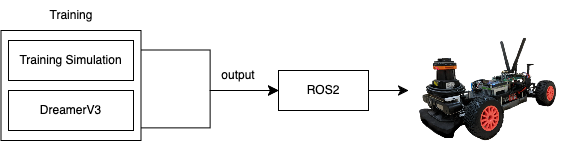
\includegraphics[scale=0.65]{deploy}
    \caption{Deployment stages}
    \label{fig:deploy}
\end{figure}

Our core objective is to pursue either the image-like conversion and the MLP-based adaptation approaches based on efficient code structures, or attempt to convert the sensor data into an image-based observation.  While the image-like conversion offers the advantage of leveraging DreamerV3's existing CNN architecture, we recognize that it might introduce information loss or require complex transformations. The MLP-based adaptation, while requiring more extensive code modifications, offers the potential for more direct and efficient processing of the LiDAR data \ref{fig:deploy}.

\section{Process}
This project follows an iterative and incremental development process, adapted from the agile methodology.  While a full-fledged agile framework with sprints and formal reviews isn't strictly necessary for this project's scale, the core principles of iterative development, continuous integration, and close collaboration seem fitting.  Our plan can be broken down into the following phases :

\begin{figure}
    \centering
    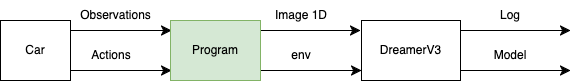
\includegraphics[scale=0.6]{program}
    \caption{Program schema}
    \label{fig:program}
\end{figure}

\begin{itemize}
    \item[1.] \textbf{Planning and Requirements Gathering (Initial Phase)}:  This initial phase involved defining the project scope, identifying key objectives, and analyzing the technical requirements.  We conducted background research, explored existing implementations, and analyzed the F1Tenth platform and its ROS2 environment \ref{fig:program}.

    \item[2.] \textbf{Design and Implementation (Iterative Cycles)}: This phase forms the core of our development process.  We adopt an iterative approach, focusing on developing and testing individual components before integrating them into the larger system.  Each iteration typically involves:
    \begin{itemize}
        \item \textbf{Component Development:} Implementing a specific module, such as the custom Gymnasium environment, the data preprocessing module, or a modification to the DreamerV3 codebase.
        \item \textbf{Unit Testing:} Thoroughly testing each component in isolation to ensure its functionality and identify potential bugs early on.
        \item \textbf{Integration:} Integrating the developed component with the existing system.
        \item \textbf{System Testing:} Testing the integrated system to ensure that the components work together correctly.
    \end{itemize}
    
    \item[3.] \textbf{Testing and Evaluation (Continuous)}: Testing is an ongoing process throughout the project.  We employ unit tests for individual components and system tests for integrated modules.  As the project progresses, we will conduct more extensive testing in the simulated F1Tenth environment to evaluate the performance of the trained agents.  This continuous testing allows us to identify and address issues early in the development cycle.
    
    \item[4.] \textbf{Documentation and Reporting (Ongoing)}: Documentation will be maintained throughout the project, with regular updates to this document, code comments, and a final project report.  This ensures that the project's progress, design decisions, and implementation details are clearly recorded.
\end{itemize}
This iterative and incremental process will provide high efficiency for this project.  It allows us to break down the complex task of integrating DreamerV3 with the F1Tenth platform into smaller, manageable units.  The continuous testing and integration enables us to identify and address issues early, preventing them from escalating into larger problems later on.  The flexibility of this approach also allows us to adapt to unforeseen challenges and adjust our plans as needed.

%\addcontentsline{toc}{chapter}{Development Process}
\chapter{Environment Set Up}

Setting up a consistent and reproducible development environment is crucial for a project of this nature.  To ensure that all team members have access to the necessary software and dependencies, and to simplify the deployment process, we have opted to use package manager UV and a virtual environment set up using the Python3 standard library. While this ensures a simpler and more stable production environment, it will require the use of local hardware resources, which are prone to compatibility issues. However, we are in active development to eliminate potential incompatibility for mainstream operating systems.

This document serves as a comprehensive guide for contributing to the DreamerV3-F1Tenth project. Whether you're interested in adding new features, fixing bugs, improving documentation, or simply sharing your expertise, this guide will provide you with the necessary information and procedures to contribute effectively.

\section{List of Packages}
We aimed to utilize the latest version of every software to enhance the compatibility among devices and reduce potential deprecation. The list of packages are extensive and continuously updated; therefore, the list will only contain the core packages that are necessary for development.
\begin{itemize}
    \item \textbf{PyTorch}: The deep learning framework used by DreamerV3.
    \item \textbf{racecar\_gym}: main gym environment forked from CPS\_TUWien.
    \item \textbf{Gymnasium}: OpenAI's gym framework used to create custom environments and standardize Machine Learning interfaces.
\end{itemize}
For more insight in installed packages, please reference uv.lock file in the root directory.

\section{Github}
This project leverages GitHub for version control, collaboration, and issue tracking.  Understanding our GitHub workflow is essential for contributing effectively.  We utilize a branching model based on Gitflow, adapted for our project's needs, to manage code changes and ensure a stable main branch.
\begin{itemize}
    \item \textbf{main Branch}: This branch represents the stable, production-ready version of the codebase.  Only reviewed and tested code is merged into main.

    \item \textbf{Feature Branches}:  These branches are created for developing new features, implementing improvements, or experimenting with new ideas.  They branch off from main and are eventually merged back into main after review.  Feature branch names should be descriptive and indicate the purpose of the branch (e.g., feature/lidar-integration, feature/mlp-world-model).

    \item \textbf{Bugfix Branches}: These branches are specifically for addressing bug fixes.  They also branch off from main and are merged back into main after the bug is resolved.  Bugfix branch names should clearly identify the bug being fixed (e.g., bugfix/incorrect-reward-calculation).

    \item \textbf{Pull Requests (PRs)}:  PRs are the mechanism for proposing changes to the main branch.  When you've completed your work on a feature or bugfix branch, you create a PR to request that your changes be reviewed and merged.

    \item \textbf{Code Review}:  Before a PR is merged, it undergoes a code review by project maintainers.  This process helps ensure code quality, identify potential issues, and promote knowledge sharing.
\end{itemize}

\section{Development Setup}
This section details the process for configuring the development environment for the DreamerV3-F1Tenth project. This setup provides a pre-configured environment containing all the necessary dependencies, including uv and the F1Tenth Gym simulator, accessible on your local machine.  This approach eliminates environment inconsistencies and simplifies the onboarding process for new contributors.

\subsection{uv Package Manager}
uv is a Python package and project manager that wraps the standard pip functionalities. We utilize uv to enhance the environment reliability. To install uv follow the guide:
\href{https://docs.astral.sh/uv/getting-started/installation/#standalone-installer}{\textcolor{blue}{uv installation guide}}

\subsection{Initial Set Up}
\begin{enumerate}
    \item Clone the repository using SSH (HTTP will not grant you access for direct commits):
    \begin{verbatim}
    git clone "git@github.com:uci-f1tenth/uci_f1tenth_workshop.git"
    \end{verbatim}
    \item Install dependencies by syncing the packages:
    \begin{verbatim}
    uv sync
    \end{verbatim}
    \item To run a file, run:
    \begin{verbatim}
    uv run path\to\file
    \end{verbatim}
    
\end{enumerate}

\subsection{Code Scheme}
The codebase is organized to clearly separate the Gym environment integration from the core DreamerV3 implementation.  This modular design facilitates maintainability and allows for independent development of each component.  The key directories and files are described below:

\begin{itemize}
    \item \texttt{dreamer\_node/agents/dreamer\_agent.py}: This is the primary file responsible for interfacing with the ROS2 environment.  It handles the subscription to the scan topic for laser scan data and the publishing of control commands (steering and speed) to the drive topic.  This file contains the logic for receiving sensor data, preprocessing it as needed, feeding it to the DreamerV3 agent, and translating the agent's actions into ROS2 messages for the F1Tenth car.
    \item \texttt{dreamer\_node/dreamer/dream.py}: This file serves as our entry point for training, orchestrating the interaction between the environment, the DreamerV3 agent, and the F1Tenth car's actuators.  The \texttt{dreamer} directory houses the DreamerV3 algorithm itself, allowing for focused development and modification of the core RL component.  This separation of concerns ensures a well-structured and easily maintainable codebase.
    \item \texttt{dreamer\_node/env/}: This directory contains the various Gymnasium environment that includes the observation space, actions space, reward functions, and step functions.
    \item \texttt{dreamer\_node/util/constants.py}: This file contains all the necessary constants and the configuration for the agent.
    
\end{itemize}

\subsection{Linters and Formatters}
By default, our Github workflow contains continuous integration that checks for correct style and formatting. We integrated \texttt{ruff} as our primary linter. If the file is not correctly formatted, any merging will be blocked by default.

\begin{itemize}
    \item To check any flags, use:
    \begin{verbatim}
    uv run ruff check
    \end{verbatim}
    \item You can also fix and error in checks with:
    \begin{verbatim}
    uv run rugg check --fix
    \end{verbatim}
    \item To auto-format the code base, use:
    \begin{verbatim}
    uv run ruff format
    \end{verbatim}
\end{itemize}



\chapter{DreamerV3}

This chapter presents a simplified and mathematically detailed implementation of the DreamerV3 algorithm, drawing inspiration from the paper "DreamerV3: Mastering Diverse Robotic Control by Dreaming"~\cite{ebert2023dreamerv3}.  We aim to provide a clear and understandable representation of the algorithm's core components and their interactions.

\section{World Model: The Agent's Internal Simulator}

The world model \ref{fig:dream}, denoted by parameters $\phi$, learns to predict the future based on current observations and actions. It's the agent's internal simulator, allowing it to "imagine" the consequences of its choices.  We use a Recurrent State-Space Model (RSSM) for this purpose.

\begin{figure}
    \centering
    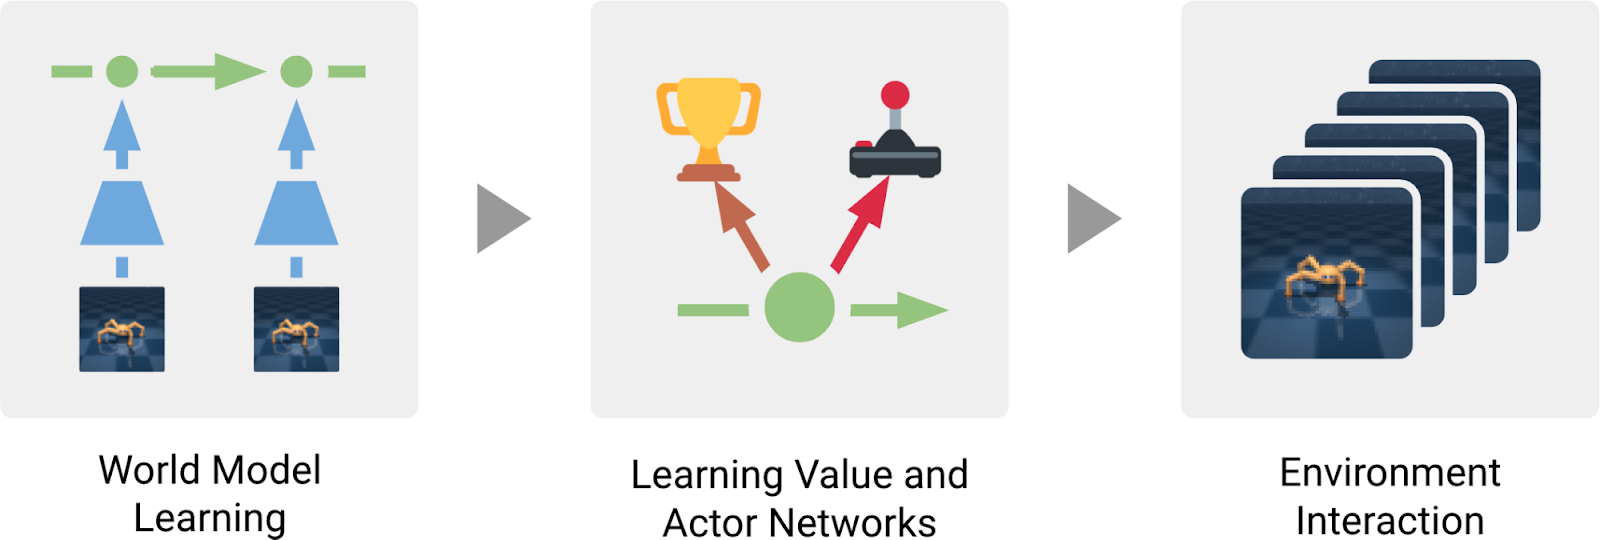
\includegraphics[scale=0.2]{dream}
    \caption{Basic functions of DreamerV3}
    \label{fig:dream}
\end{figure}

\subsection{RSSM Components}

\begin{enumerate}
    \item \textbf{Encoder:} Takes the current observation (sensory input) $x_t$ and the previous hidden state $h_{t-1}$ and produces a latent state $z_t$. This is a probabilistic mapping:
        \begin{equation}
            z_t \sim q_\phi(z_t | h_{t-1}, x_t)
        \end{equation}
        We can think of $q_\phi$ as a neural network (e.g., a multilayer perceptron or a convolutional network if $x_t$ is an image) parameterized by $\phi$.

    \item \textbf{Recurrent Dynamics Model:} Predicts the next hidden state $h_t$ based on the previous hidden state $h_{t-1}$, the previous latent state $z_{t-1}$, and the action taken $a_{t-1}$:
        \begin{equation}
            h_t = f_\phi(h_{t-1}, z_{t-1}, a_{t-1})
        \end{equation}
        $f_\phi$ is another neural network (e.g., an RNN or LSTM).

    \item \textbf{Dynamics Predictor:} Predicts the next latent state $\hat{z}_t$ based on the current hidden state $h_t$:
        \begin{equation}
            \hat{z}_t \sim p_\phi(\hat{z}_t | h_t)
        \end{equation}

    \item \textbf{Reward Predictor:} Predicts the reward $\hat{r}_t$ the agent expects to receive:
        \begin{equation}
            \hat{r}_t \sim p_\phi(\hat{r}_t | h_t, z_t)
        \end{equation}

    \item \textbf{Continue Predictor:} Predicts whether the episode will continue ($\hat{c}_t = 1$) or terminate ($\hat{c}_t = 0$):
        \begin{equation}
            \hat{c}_t \sim p_\phi(\hat{c}_t | h_t, z_t)
        \end{equation}

    \item \textbf{Decoder:} Reconstructs the observation $\hat{x}_t$ from the latent state $z_t$ and hidden state $h_t$:
        \begin{equation}
            \hat{x}_t \sim p_\phi(\hat{x}_t | h_t, z_t)
        \end{equation}
\end{enumerate}

\subsection{World Model Loss}

The world model is trained by minimizing the following loss function:

\begin{equation}
L_{WM}(\phi) = \sum_{t=1}^T \left[ L_{pred}(t) + L_{dyn}(t) + \lambda_{rep} L_{rep}(t) \right]
\end{equation}

where $\lambda_{rep}$ is a weighting factor (e.g., 0.1). The individual loss terms are:

\begin{align}
L_{pred}(t) &= -\log p_\phi(x_t | z_t, h_t) - \log p_\phi(r_t | z_t, h_t) - \log p_\phi(c_t | z_t, h_t) \\
L_{dyn}(t) &= \max\left(1, KL\left(q_\phi(z_t | h_{t-1}, x_t) || p_\phi(z_t | h_t)\right)\right) \\
L_{rep}(t) &= \max\left(1, KL\left(q_\phi(z_t | h_{t-1}, x_t) || p_\phi(z_t | h_t)\right)\right)
\end{align}

The KL divergence term encourages the approximate posterior $q_\phi$ to be close to the prior $p_\phi$. The $\max(1, \cdot)$ term implements the "free bits" technique.

\section{Critic: Evaluating the Agent's Performance}

The critic, parameterized by $\psi$, learns to estimate the expected cumulative reward (return) from a given state. The critic network $v_\psi(s_t)$ takes the state $s_t = (h_t, z_t)$ as input and outputs a prediction of the return.  It is trained to predict the distribution of returns.

The critic is trained using the following loss function:

\begin{equation}
L_C(\psi) = \sum_{t=1}^T -\log p_\psi(R_t^\lambda | s_t)
\end{equation}

where $R_t^\lambda$ is the $\lambda$-return, calculated as:

\begin{align}
R_t^\lambda &= r_t + \gamma c_t \left( (1-\lambda) v_\psi(s_t) + \lambda R_{t+1}^\lambda \right) \\
R_T^\lambda &= v_\psi(s_T)
\end{align}

$\gamma$ is the discount factor, and $\lambda$ controls the balance between bootstrapping and using the actual returns.

\section{Actor: Choosing the Optimal Actions}

The actor, parameterized by $\theta$, learns to select actions that maximize the expected return. The actor network $\pi_\theta(a_t | s_t)$ takes the state $s_t$ as input and outputs a probability distribution over actions. The actor is trained using the following loss function:

\begin{equation}
L_A(\theta) = \sum_{t=1}^T - \frac{R_t^\lambda - v_\psi(s_t)}{\max(1, S)} \log \pi_\theta(a_t | s_t) + \eta H(\pi_\theta(a_t | s_t))
\end{equation}

where $S$ is a running average of the range of returns (between the 5th and 95th percentiles), and $\eta$ is the entropy bonus coefficient.  This loss function combines maximizing returns with encouraging exploration.

\section{Symlog Transformation and Twohot Encoding}

DreamerV3 uses the symlog transformation to handle rewards and observations with different scales. The symlog function is defined as:

\begin{equation}
\text{symlog}(x) = \text{sign}(x) \log(|x| + 1)
\end{equation}

Its inverse, the symexp function, is:

\begin{equation}
\text{symexp}(x) = \text{sign}(x) (\exp(|x|) - 1)
\end{equation}

For rewards and returns, DreamerV3 uses a categorical distribution with exponentially spaced bins and twohot encoding.  This allows the model to predict continuous values while maintaining stable gradients.

This simplified mathematical description provides a more accessible understanding of the DreamerV3 algorithm.  It clarifies the roles of each component and their interactions, highlighting the key mathematical operations involved.  This foundation should be helpful for implementing and adapting DreamerV3 for various robotic control tasks.
\chapter{Understanding F1Tenth ROS Control}

This chapter provides a detailed explanation of how the F1Tenth autonomous racing car interacts with ROS 2 using a simple wall following example written in Python.  We will dissect the code, explaining the purpose of each section and how it relates to the overall ROS 2 communication and control process.

\section{Code Overview}

The provided Python code implements a wall following algorithm for the F1Tenth car. It uses a Proportional-Integral-Derivative (PID) controller to maintain a desired distance from a wall.  The code interacts with the simulator through ROS 2 topics such as \ref{fig:ros}.

\subsection{ROS 2 Node and Topic Setup}

The code defines a ROS 2 node named \texttt{wall\_follow\_node}.  This node subscribes to the \texttt{/scan} topic, which publishes \texttt{LaserScan} messages containing LiDAR data, and publishes to the \texttt{/drive} topic, which accepts \texttt{AckermannDriveStamped} messages to control the car's steering and speed.

\begin{figure}
    \centering
    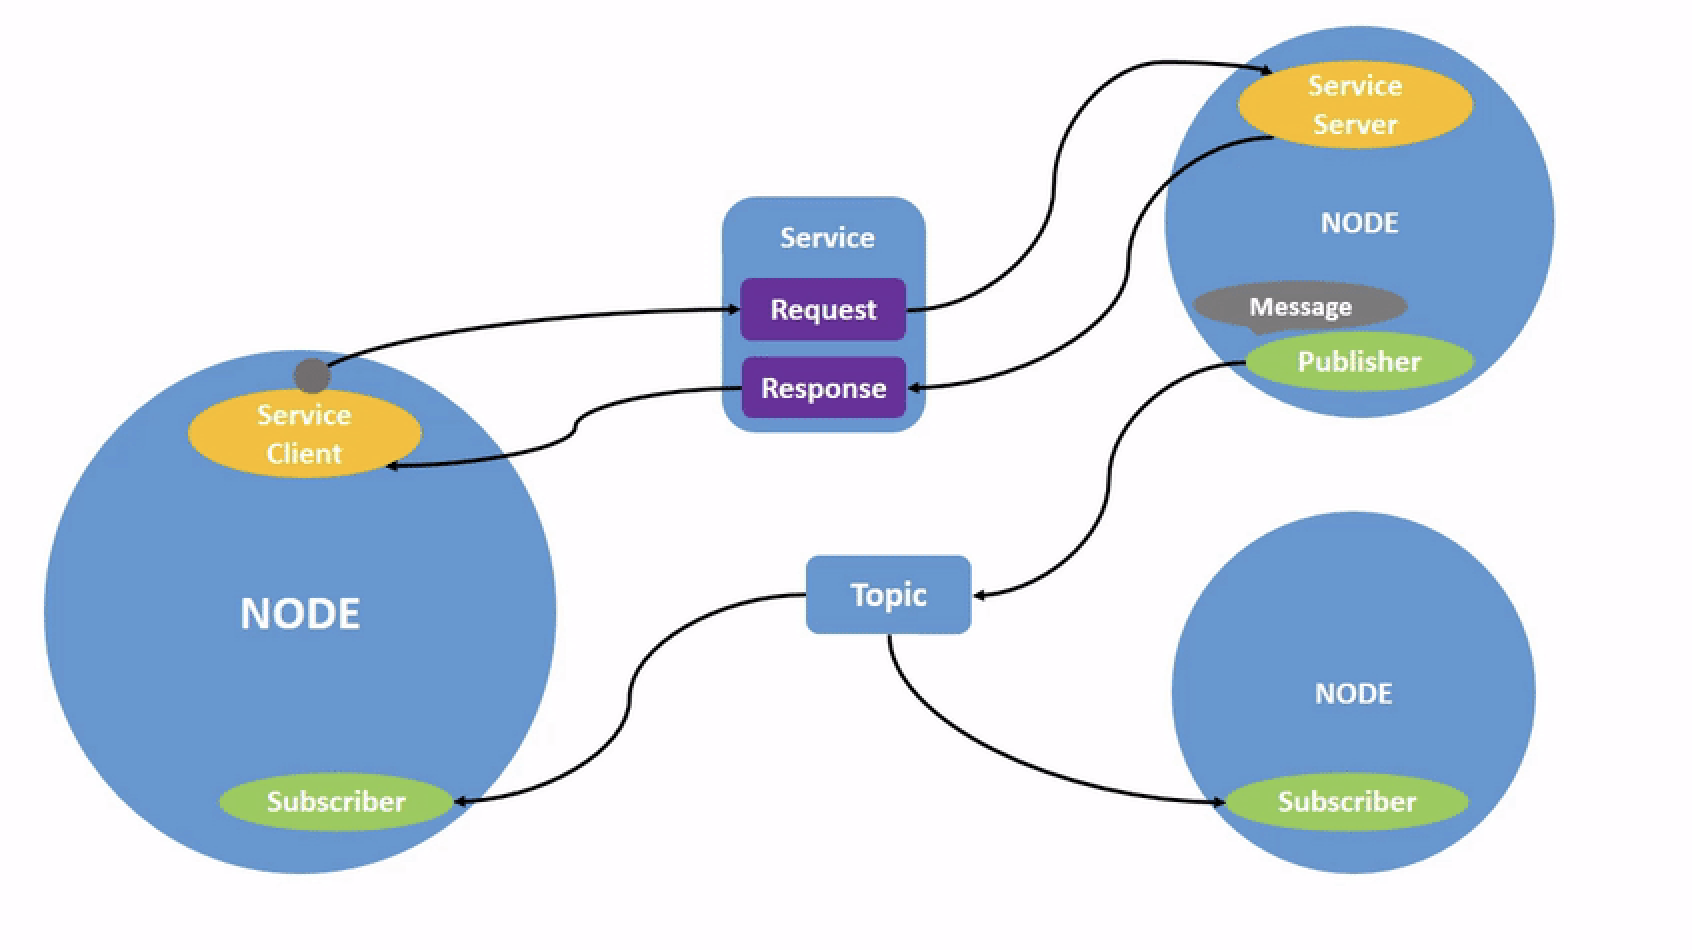
\includegraphics[scale=0.2]{ROS2}
    \caption{Basic ROS2 workflow}
    \label{fig:ros}
\end{figure}

\begin{verbatim}
lidarscan_topic = '/scan'
drive_topic = '/drive'

self.sub_scan = self.create_subscription(LaserScan, ...
self.pub_drive = self.create_publisher(AckermannDriveStamped, ...
\end{verbatim}

These lines of code set up the communication channels.  \texttt{self.create\_subscription} creates a subscriber that listens for \texttt{LaserScan} messages on the \texttt{/scan} topic and calls the \texttt{scan\_callback} function whenever a new message arrives.  \texttt{self.create\_publisher} creates a publisher that sends \texttt{AckermannDriveStamped} messages on the \texttt{/drive} topic to control the car.

\subsection{Helper Functions}

The code includes helper functions to process the LiDAR data and calculate the error.

\subsubsection{\texttt{get\_range(range\_data, angle)}}

This function takes the raw LiDAR data and an angle as input and returns the corresponding range measurement at that angle. It handles potential \texttt{NaN} (Not a Number) and \texttt{inf} (infinity) values in the LiDAR data.

\subsubsection{\texttt{get\_error(range\_data, dist)}}

This function calculates the error, which is the difference between the desired distance to the wall (\texttt{dist}) and the actual distance calculated from the LiDAR data.  It uses geometric calculations based on LiDAR readings at specific angles to estimate the distance to the wall.

\subsection{PID Control}

The \texttt{pid\_control} function implements the PID controller.  It takes the calculated error, desired velocity, time difference (\texttt{delta\_t}), and some additional LiDAR beam measurements as input.  It calculates the steering angle based on the PID gains (\texttt{kp}, \texttt{ki}, \texttt{kd}) and publishes the control command to the \texttt{/drive} topic.  The code also includes a simple obstacle avoidance mechanism based on the front LiDAR beam.

\begin{verbatim}
self.integral += self.ki * self.error * delta_t
angle = self.kp * self.error + np.clip(self.integral, -1, +1) ...

drive_msg.drive.speed = velocity
drive_msg.drive.steering_angle = angle
self.pub_drive.publish(drive_msg)
\end{verbatim}

This section calculates the PID output (steering angle) and publishes it along with the desired speed as an \texttt{AckermannDriveStamped} message.

\subsection{Scan Callback}

The \texttt{scan\_callback} function is the heart of the wall following algorithm.  It is called every time a new \texttt{LaserScan} message is received.  This function performs the following steps:

\begin{enumerate}
    \item Calculates the time elapsed since the last message.
    \item Calls \texttt{get\_error} to calculate the error.
    \item Calculates the desired car velocity based on the current heading angle.
    \item Calls \texttt{pid\_control} to calculate the steering angle and publish the drive message.
    \item Updates the previous time.
\end{enumerate}

\subsection{Main Function}

The \texttt{main} function initializes the ROS 2 node, creates the \texttt{WallFollow} object, and starts the ROS 2 event loop using \texttt{rclpy.spin()}.  This keeps the node alive and processes incoming messages. The final result of the program should look something like this: \ref{fig:struct}

\begin{figure}
    \centering
    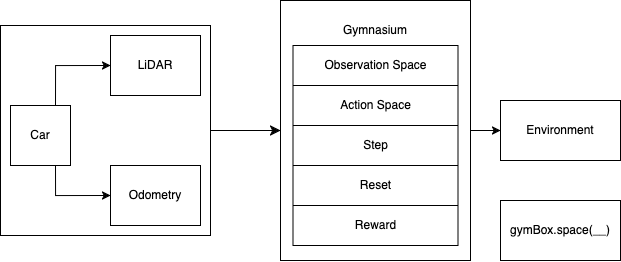
\includegraphics[scale=0.5]{structure}
    \caption{Structure of the program}
    \label{fig:struct}
\end{figure}

\section{ROS 2 Communication Flow}

The LiDAR sensor data is published on the \texttt{/scan} topic.  The \texttt{wall\_follow\_node} subscribes to this topic, processes the data, and publishes control commands on the \texttt{/drive} topic.  The F1Tenth car's actuators subscribe to the \texttt{/drive} topic and execute the commands.

This example demonstrates a basic ROS 2 node that interacts with sensor data and publishes control commands. It showcases the fundamental concepts of ROS 2 communication and provides a foundation for more complex autonomous driving algorithms.
\chapter{Implementation Details}

This chapter details the core logic behind integrating the F1tenth autonomous race car with the DreamerV3 reinforcement learning agent. It explains the structure of the DreamerV3 codebase, how we adapt it for the F1tenth platform using ROS2 Humble, the importance of data type compatibility and normalization, and outlines the high-level implementation goals and timeline.

\section{DreamerV3 Codebase Structure}

The DreamerV3 codebase is designed with a hyperparameter-driven approach, with its main function located in \texttt{dream.py}.  It utilizes OpenAI Gymnasium environments to define the observation space, action space, the \texttt{step()} function (which interacts with the environment), and the \texttt{reset()} function (to reset the environment).  Wrappers are employed to configure these environments and perform necessary data preprocessing.

A typical DreamerV3 environment definition looks like this (example from the Crafter environment):

\begin{verbatim}
import gym
import numpy as np

class Crafter:
    # ... (metadata and initialization) ...

    @property
    def observation_space(self):
        # ... (defines the structure of the observation) ...

    @property
    def action_space(self):
        # ... (defines the structure of the action) ...

    def step(self, action):
        # ... (interacts with environment based on action) ...

    def reset(self):
        # ... (resets the underlying environment) ...
\end{verbatim}

Wrappers, like the `NormalizeActions` wrapper in the DreamerV3 examples, can be used to modify the environment (like normalizing the action space).

\section{Adapting DreamerV3 for F1tenth with ROS2 Humble}

Our primary goal is to replace the standard DreamerV3 environment (like Crafter) with an interface to the F1tenth car within the ROS2 Humble framework.  This involves creating a custom Gymnasium environment, \texttt{racerenv.py}, that acts as a bridge between DreamerV3 and ROS2.  This environment will not directly handle ROS2 communication.  Instead, a separate ROS2 node, \texttt{dreamer\_node.py}, will manage all ROS2 interactions (subscribing to LiDAR and Odometry data, publishing motor commands) and pass the processed data to \texttt{racerenv.py}.

\subsection{Data Flow and Compatibility}

The \texttt{dreamer\_node.py} will subscribe to the relevant ROS2 topics:
\begin{itemize}
    \item \texttt{/scan}:  For LiDAR data.
    \item \texttt{/odom}: For Odometry data.
    \item \texttt{/drive}: To publish drive commands.
\end{itemize}

The \texttt{dreamer\_node.py} will then process the received ROS2 messages.  The LiDAR data (a 1D array of floats) and Odometry data will be extracted and passed to the \texttt{racerenv.py}'s \texttt{step()} and \texttt{reset()} methods.  The actions generated by the DreamerV3 agent will be passed from \texttt{racerenv.py} to \texttt{dreamer\_node.py}, which will then publish them as messages to the \texttt{/drive} topic.

\subsection{Data Normalization}

Data normalization is crucial for stable and effective reinforcement learning.  Raw sensor data (LiDAR, Odometry) often has a wide range of values, which can make it difficult for the agent to learn.  We normalize the LiDAR data to a range of [0, 1] within the \texttt{racerenv.py} environment.  The action space (steering and speed) is also normalized to a range of [-1, 1]. This ensures that both the input and output of the DreamerV3 agent are within a consistent and manageable range.  The denormalization of the actions (from [-1,1] to the cars physical limits) happens in the `step` function before being published to the car.

\section{Implementation Goals and Timeline}

Our primary goals for this project are:

\begin{itemize}
    \item Create a robust and efficient interface between the F1tenth car and DreamerV3.
    \item Train the DreamerV3 agent to successfully navigate the F1tenth car in various simulated environments.
    \item Evaluate the performance of the trained agent using appropriate metrics.
    \item Document the project thoroughly.
\end{itemize}

The project timeline is divided into the following phases:

\begin{enumerate}
    \item \textbf{Environment and ROS2 Integration:} Implementing \texttt{racerenv.py} and \texttt{dreamer\_node.py}, establishing ROS2 communication.
    \item \textbf{DreamerV3 Adaptation:} Integrating \texttt{racerenv.py} with the DreamerV3 training loop, adapting networks.py, implementing the reward function.
    \item \textbf{Isaac Lab Migration}: Migration to Isaac Lab since F1Tenth Gym is proved to be unreliable.
    \item \textbf{Training and Evaluation:} Training the agent, tuning hyperparameters, evaluating performance in simulation.
    \item \textbf{Testing and Refinement:} Testing in more complex scenarios, refining the code, and documenting the project.
\end{enumerate}

This timeline is subject to change based on project progress and any unforeseen challenges.  Regular team meetings and communication will be essential to ensure the project stays on track.
% add any additional chapters here

\end{document}
